\chapter{Riconoscitore di sequenze}

\section{Riconoscitore di sequenze}
\paragraph{Traccia}
Progettare, implementare in VHDL e testare mediante simulazione una macchina in grado di riconoscere la sequenza 1001. La macchina prende in ingresso un segnale binario i che rappresenta il dato, un segnale A di tempificazione e un segnale M di modo, che ne disciplina il funzionamento, e fornisce un’uscita Y alta quando la sequenza viene riconosciuta. In particolare, 
-	se M=0, la macchina valuta i bit seriali in ingresso a gruppi di 4, 
-	se M=1, la macchina valuta i bit seriali in ingresso uno alla volta, tornando allo stato iniziale ogni volta che la sequenza viene correttamente riconosciuta.


\subsection{Architettura}
Data la natura sequenziale del problema è stato realizzato un automa a stati finiti di cui è possibile vedere lo schema in Figura \ref{fig: automa_3.1}.

\begin{figure}[H]
    \centering
    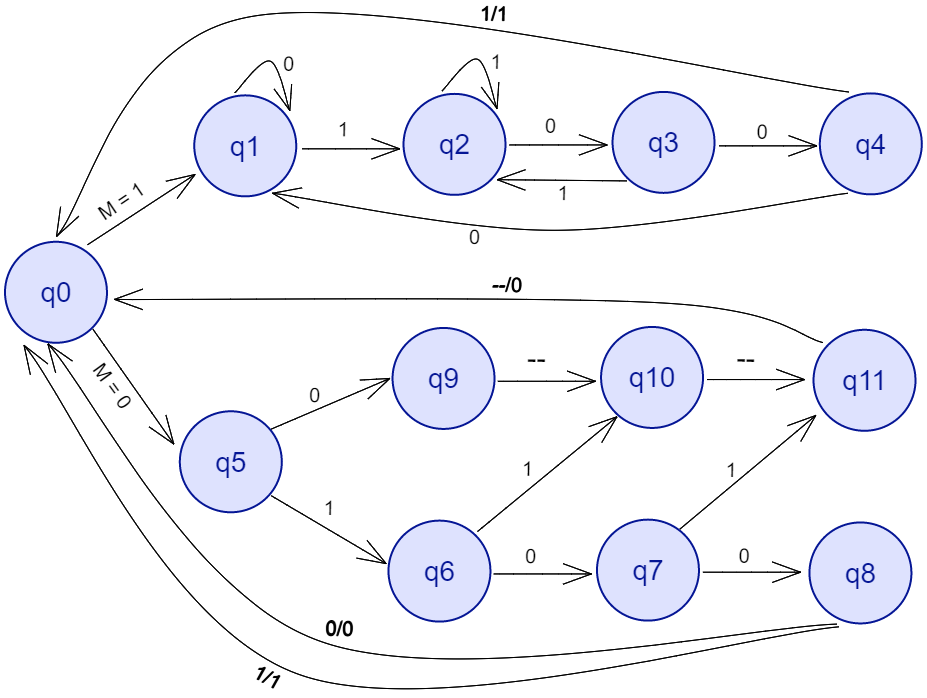
\includegraphics[width=14cm]{immagini/esercizio3/schema_3.1.png}
    \caption{Schema della soluzione}
    \label{fig: automa_3.1}
\end{figure}


Essendo una macchina sequenziale, è stato descritto il funzionamento dell'automa, dividendo la parte combinatoria da quella sequenziale. È stato esaminato il comportamento della macchina in ogni stato, in base agli input e, inoltre, è stato descritto il funzionamento del clock.
La macchina può funzionare in due diverse modalità, rappresentate dalle diramazioni che partono dagli stati \textbf{$q_1$} e \textbf{$q_5$}. Per poter scegliere tra le due si imposta il \textbf{modo} M nel primo stato \textbf{$q_0$}. É da notare che è possibile cambiare il modo solamente partendo da \textbf{$q_0$}, per cui si hanno due opzioni: o si aspetta che la sequenza venga riconosciuta e quindi si torna a \textbf{$q_0$} auromanticamente, oppure è necessario utilizzare il segnale di \textbf{reset}. Questo comportamento è stato scelto in modo da garantire l'integrità del riconoscimento una volta avviato, e inoltre permette di semplificare la logica interna agli stati non dovendo gestire sempre il modo.

 L'implementazione dell'automa, nel listato di codice \ref{riconoscitore_sequenza}, prevede la separazione della componente combinatoria, quella che sceglie in quale stato andare in base agli input e imposta gli output, da quella sequenziale, che si occupa dell'effettivo cambio di stato. 
 Sono infatti presenti due processi diversi. Nel primo viene utilizzato il costrutto \textit{case when} per definire gli stati e i possibili input, per cui la \textit{sensitivity list} comprende lo stato corrente e i dati in ingresso. Il secondo è invece attivato solo dal clock, presente nella sensitivity list, ed a ogni fronte di salita cambia lo stato corrente con il prossimo. É stato utilizzato un reset sincrono, infatti il segnale di reset è assente dalla lista di sensitività. In questo modo il reset allo stato \textit{$s_0$} avverrà in maniera sincronizzata con il clock.
\begin{lstlisting} [language=VHDL, label=riconoscitore_sequenza, caption=Riconoscitore di sequenze]
library IEEE;
use IEEE.STD_LOGIC_1164.ALL;

entity riconoscitore_sequenza is
    Port(
        i: in std_logic;
        A: in std_logic;
        RST: in std_logic;
        M: in std_logic; 
        Y: out std_logic          
    );
end riconoscitore_sequenza;

architecture Behavioral of riconoscitore_sequenza is

type stato is (S0, S1, S2, S3, S4, S5, S6, S7, S8, S9, S10, S11);
signal stato_corrente : stato:= S0;
signal stato_prossimo : stato;

begin

  f_stato_uscita: process(stato_corrente,i) 
    begin
    case stato_corrente is 
    
        when S0=>
            if(M='0') then
                stato_prossimo<=S5;
                Y<='0';
            else
                stato_prossimo<=S1;
                Y<='0';
            end if;
    
        when S1=>
            if(i='0') then
                stato_prossimo<=S1;
                Y<='0';
            else
                stato_prossimo<=S2;
                Y<='0';
            end if;
    
         when S2=>
            if(i='0') then
                stato_prossimo<=S3;
                Y<='0';
            else
                stato_prossimo<=S2;
                Y<='0';
            end if;   

         when S3=>
            if(i='0') then
                stato_prossimo<=S4;
                Y<='0';
            else
                stato_prossimo<=S2;
                Y<='0';
            end if;   

         when S4=>
            if(i='0') then
                stato_prossimo<=S1;
                Y<='0';
            else
                stato_prossimo<=S0;
                Y<='1';
            end if;        
            
         when S5=>
            if(i='0') then
                stato_prossimo<=S9;
                Y<='0';
            else
                stato_prossimo<=S6;
                Y<='0';
            end if;               
    
         when S6=>
            if(i='0') then
                stato_prossimo<=S7;
                Y<='0';
            else
                stato_prossimo<=S10;
                Y<='0';
            end if;       
    
          when S7=>
            if(i='0') then
                stato_prossimo<=S8;
                Y<='0';
            else
                stato_prossimo<=S11;
                Y<='0';
            end if;      
    
          when S8=>
            if(i='0') then
                stato_prossimo<=S0;
                Y<='0';
            else
                stato_prossimo<=S0;
                Y<='1';
            end if;      
    
          when S9=>
            if(i='0') then
                stato_prossimo<=S10;
                Y<='0';
            else
                stato_prossimo<=S10;
                Y<='0';
            end if;      
    
           when S10=>
            if(i='0') then
                stato_prossimo<=S11;
                Y<='0';
            else
                stato_prossimo<=S11;
                Y<='0';
            end if;   
    
           when S11=>
            if(i='0') then
                stato_prossimo<=S0;
                Y<='0';
            else
                stato_prossimo<=S0;
                Y<='0';
            end if;     
        end case;
    end process;
    
    mem: process(A)
    begin 
        if (A'event and A='1') then
            if(RST='1')then 
                stato_corrente<=S0;
            else
            stato_corrente<=stato_prossimo;  
            end if;
        end if;
    end process;
end Behavioral;
\end{lstlisting}

\subsection{Testing}

In primo luogo è stata effettuata una wait di 100 ns per aspettare che il segnale di GRS (Global Set Reset) diventasse alto ed è stata resettata la macchina. Sono stati verificati quattro casi di test.
I primi tre casi di test sono stati effettuati impostando il modo a 0, ovvero riconoscendo la sequenza a gruppi di 4. Nel primo è stato inserito in input la sequenza corretta, negli altri due la sequenza errata. In particolare, la sequenza errata è stata inserita in modo che il sistema fosse in grado di riconoscere lo stato errato della modalità 1. 
Infine, l'ultimo caso di test è stato effettuato impostando il modo a 1, ovvero il sistema deve essere in grado di riconoscere la sequenza all'interno di un generico blocco. Dopo una serie di bit errati misti a quelli corretti si giunge al riconoscimento. All'interno della schermata di simulazione sono stati aggiunti gli stati prossimi e correnti dell'automa, in modo da tracciarne l'evoluzione.

I casi di test sono stati realizzati con il seguente codice:

\begin{lstlisting} [language=VHDL, caption=Testbench example]
library IEEE;
use IEEE.STD_LOGIC_1164.ALL;

entity riconoscitore_sequenza_TB is
end riconoscitore_sequenza_TB;

architecture Behavioral of riconoscitore_sequenza_TB is

    component riconoscitore_sequenza is
        Port(
            i: in std_logic;
            A: in std_logic;
            RST: in std_logic;
            M: in std_logic;
            Y: out std_logic
        );
    end component;

    signal input: std_logic:= '0';
    signal clock: std_logic:= '0';
    signal reset: std_logic:= '0';
    signal mode: std_logic:= '0';
    signal output: std_logic;
    constant CLK_period : time := 10 ns;

begin
    uut: riconoscitore_sequenza
        port map(
            i=>input,
            A=>clock,
            RST=>reset,
            M=>mode,
            Y=>output
        );

    CLK: process
    begin
        clock<='0';
        wait for CLK_period/2;
        clock<='1';
        wait for CLK_period/2;
    end process;

    RS_TB: process
    begin
        wait for 100 ns;
        reset<='1';
        wait for 10 ns;
        reset<='0';

        mode<='0'; 
        -- Caso di test 1
        wait for 10ns;
        input<='1';
        wait for 10ns;
        input<='0';
        wait for 10ns;
        input<='0';
        wait for 10ns;
        input<='1';
        wait for 5ns;
        assert output='1' 
        report "errore modo 0 caso 1";
        wait for 5ns;

        -- Caso di test 2
        input<='1';
        wait for 10ns;
        input<='1';
        wait for 10ns;
        input<='0';
        wait for 10ns;
        input<='0';
        wait for 10ns;
        input<='0';
        wait for 5ns;
        assert output='0'
        report "errore modo 0 caso 2";
        wait for 5ns;

        --Caso di test 3
        input<='1';
        wait for 10ns;
        input<='1';
        wait for 10ns;
        input<='1';
        wait for 10ns;
        input<='1';
        wait for 10ns;
        
        mode<='1';
        -- Caso di test 4
        wait for 10ns;
        input<='1';
        wait for 10ns;
        input<='1';
        wait for 10ns;
        input<='0';
        wait for 10ns;
        input<='0';
        wait for 10ns;
        input<='1';
        wait for 5ns;
        assert output='1'
        report "errore modo 1 caso 3";
        wait for 5ns;
        
        wait;
    end process;
end Behavioral;
\end{lstlisting}

\begin{figure}[H]
    \centering
    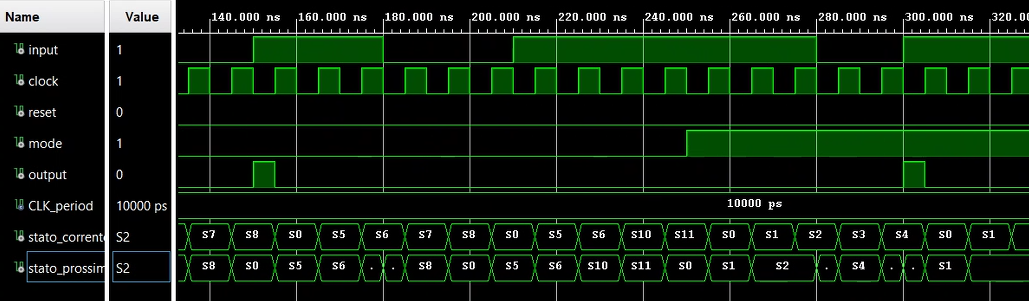
\includegraphics[width=16cm]{immagini/esercizio3/output_simulazione_3.1.png}
    \caption{Output della simulazione}
\end{figure}


\section{Sintesi su scheda}
\paragraph{Traccia}
Sintetizzare e implementare su board la rete sviluppata al punto precedente, utilizzando uno switch S1 per codificare l’input i e uno switch S2 per codificare il modo M, in combinazione con due bottoni B1 e B2 utilizzati rispettivamente per acquisire l’input da S1 e S2 in sincronismo con il segnale di tempificazione A, che deve essere ottenuto a partire dal clock della board. Infine, l’uscita Y può essere codificata utilizzando un led.

\subsection{Implementazione}
Per poter sintetizzare e implementare sulla board la soluzione simulata è stato innanzitutto necessario gestire gli input provenienti dai bottoni. Per farlo sono stati utilizzati due \textit{debouncer}, impostati entrambi con il clock della scheda. Per fornire a tutti i componenti il clock reale del dispositivo sono state decommentate le due righe opportune sul file dei costraint, specificando il nome del segnale utilizzato. La scheda fornisce un clock di 100Mhz, come descritto nei capitoli precedenti, i debouncer "puliscono" i segnali in entrata dai pulsanti in modo che possano essere letti correttamente dai componenti del sistema . Infine sono stati mappati il primo switch all'input e il primo led all'uscita. 
Nel file \textit{video 3.2} presente nel materiale multimediale è possibile vedere il funzionamento della scheda con un caso di test. In particolare, viene impostata in modalità 1 e viene inserita la sequenza corretta da riconoscere. 

Di seguito è mostrato il codice relativo al componente che ingloba tutti gli altri per la sintetizzazione sulla scheda.
È stato utilizzato il riferimento diretto al file sorgente senza l'uso del component.


\begin{lstlisting} [language=VHDL, caption=Testbench example]
library IEEE;
use IEEE.STD_LOGIC_1164.ALL;

entity top_scheda is
    port(
        x      : in std_logic;
        clk    : in std_logic;
        rst    : in std_logic;
        mode     : in std_logic;
        set_mode: in std_logic;
        set_x: in std_logic;
        y    : out std_logic
    );
end top_scheda;

architecture Behavioral of top_scheda is
    signal seq_en: std_logic := '0';
    signal db_set_m, db_set_x : std_logic := '0';
begin

   seq_r: entity work.riconoscitore_sequenza port map(
            clk=>clk,
            en => seq_en,
            rst => rst,
            mode=>mode,
            y=>y,
            x=>x
        );
    
    ctrl_unit: entity work.cu port map (
        clk => clk,
        rst =>rst,
        set_mode=> db_set_m,
        set_x => db_set_x,
        seq_en => seq_en
    );
    dbnc_set_m: entity work.debouncer port map (
        clk=>clk,
        rst=>rst,
        btn=>set_mode,
        cleared_btn => db_set_m
    );
    
      dbnc_set_x: entity work.debouncer port map (
        clk=>clk,
        rst=>rst,
        btn=>set_x,
        cleared_btn => db_set_x
    );

end Behavioral;
\end{lstlisting}